\frame
{
  \frametitle{An approach using Piecewise Linear modeling}

}

 \frame
{
  \frametitle{Ideal Diode}
   \centerline{
  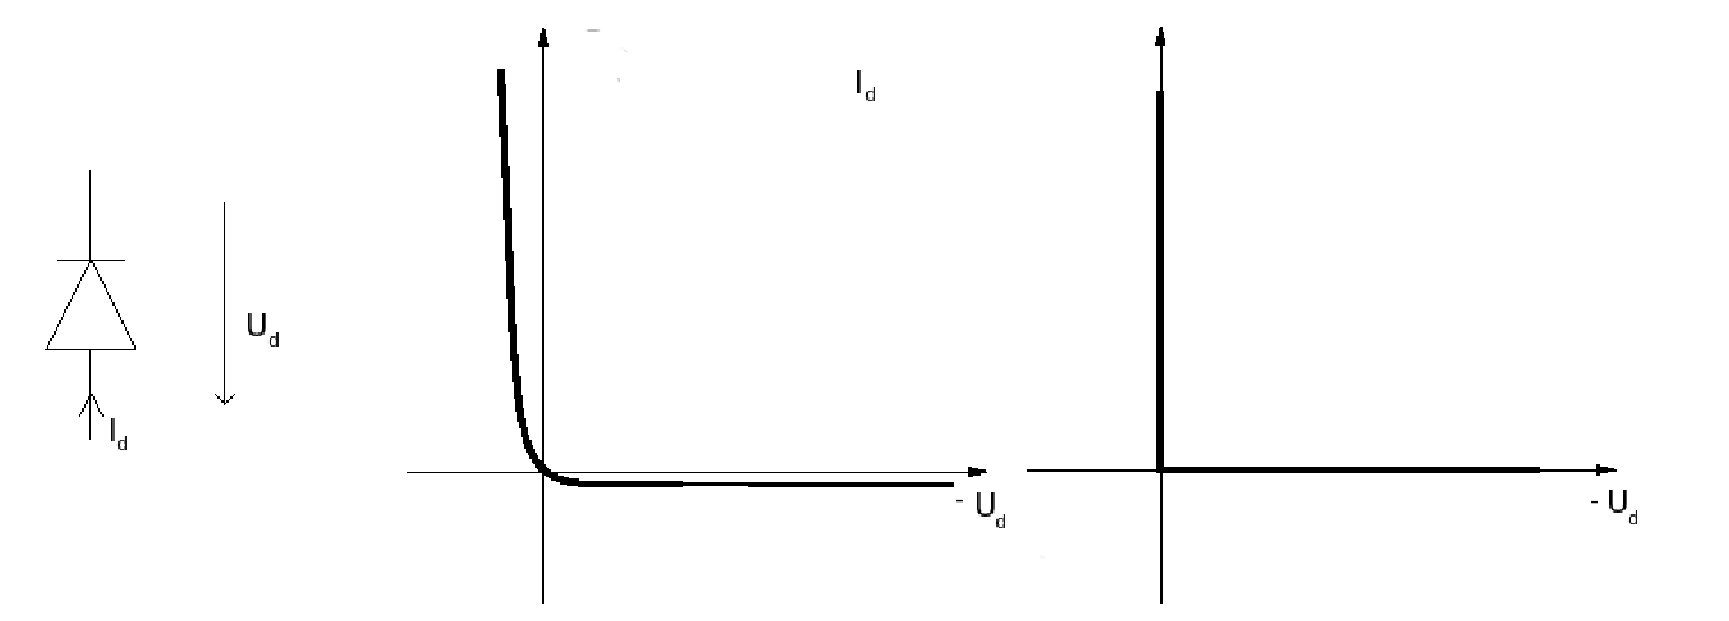
\includegraphics[width=100mm]{diode.eps}
  }
   \begin{block}{Branch Constitutive Equation of the diode:}
  \[ I_d =I_{s}(\exp{(-U_{D}/C)}-1)\]
  \end{block}
   \begin{block}{The complementary formulation:}
  \[0 \leq I_d \, \perp \, -U_{D} \geq 0\]
  \end{block}

}
\frame
{
  \frametitle{Ideal Transistor}
   \centerline{
  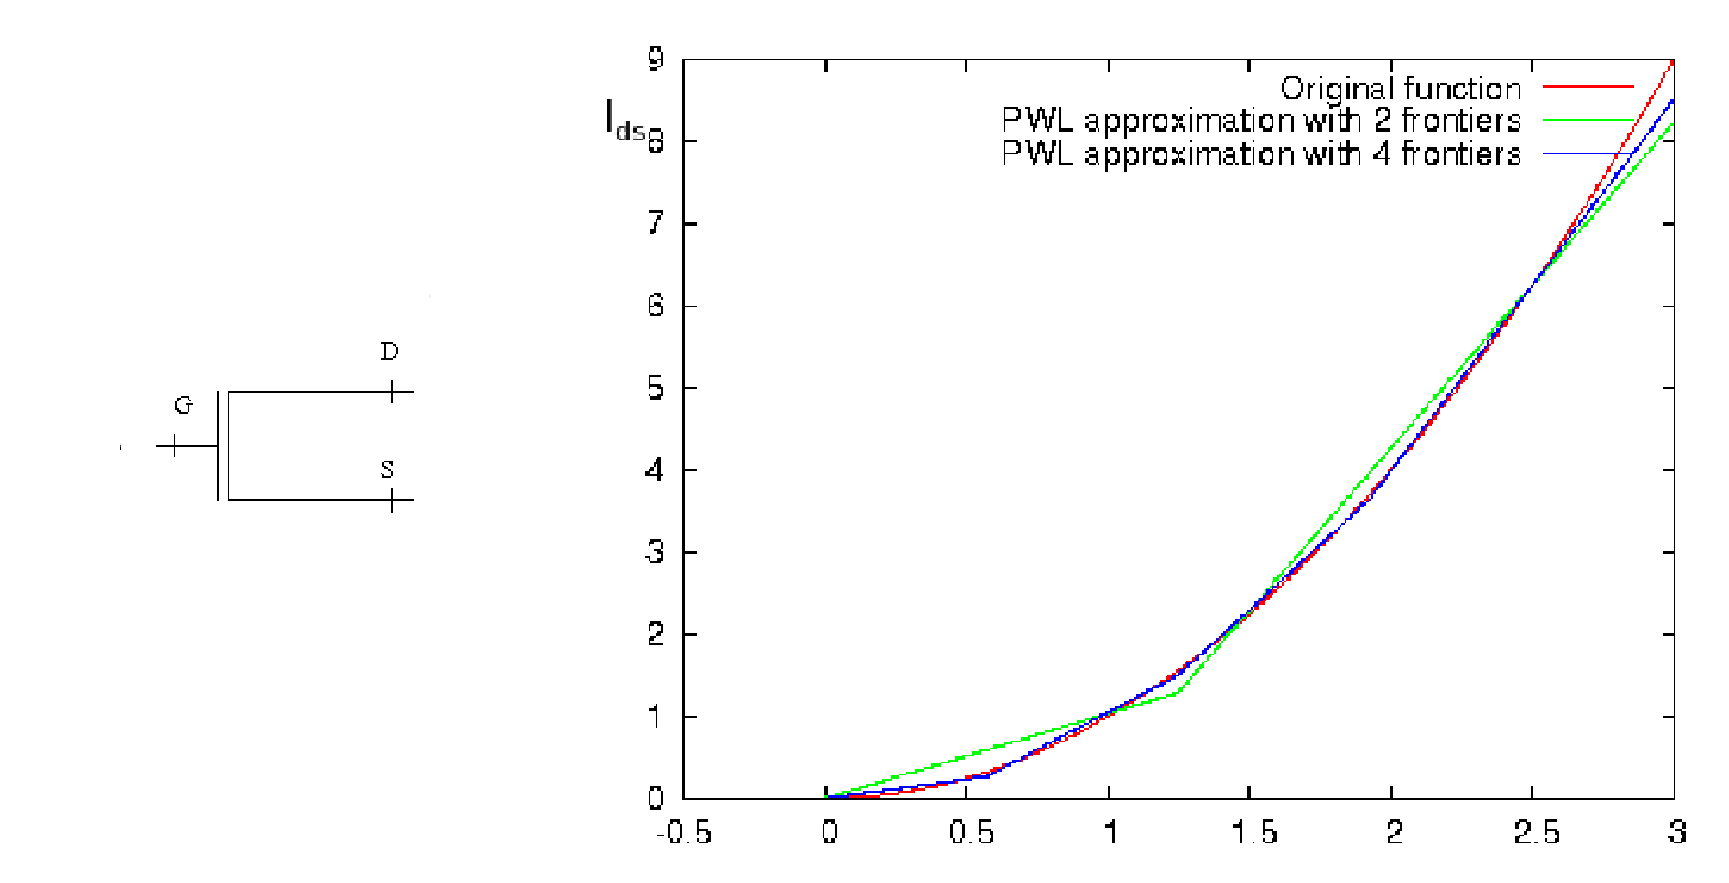
\includegraphics[width=100mm]{def2.eps}
  }
   \begin{block}{The complementary formulation:}
  \[ I_{d} = \left(\begin{array}{ccc}
  c_{1}&...&c_{10}\end{array}\right)\lambda \qquad  I_{d} = -I_{s}\]
  \[Y=A\left(\begin{array}{c}
  V_{d}\\
  V_{g}\\
  V_{s}\\\end{array}\right)+I\lambda + C\]
  \[0 \leq Y \, \perp \, \lambda \geq 0\]
  \end{block}

}
 
 \frame
{
\frametitle{Complementarity formulation.}

\begin{figure}
   \centerline{
   \scalebox{0.8}{
    \input{CSsmall.pstex_t}
    }
 } 
 \end{figure}

  
 \begin{eqnarray*}
 &{\color{Green}L\dot I_L -(V_1-V_2)=0}&V_3-e(t)=0\\
 &I_L-I_S-I_D=0&RI_L-V_2=0\\
 &{\color{Red}V_1+I_D(\lambda _4 +R_{on})}&{\color{Blue}V_1-20+I_S(\lambda _2 - R_{on})=0}\\
 &{\color{Red}y_3=R_{off}-\lambda _4 - R_{on}}&{\color{Blue}y_1=R_{off}-\lambda _2-R_{on}}\\
 &{\color{Red}y_4=-V_1+\lambda _3}&{\color{Blue}y_2=V_3-V_2+\lambda _1}\\
 \end{eqnarray*}
 \[0 \leq y_i \perp \lambda _i \geq 0\]
 }

\frame
{

\frametitle{Complementarity formulation.}
 \begin{figure}
 %GNUPLOT: LaTeX picture with Postscript
\begin{picture}(0,0)%
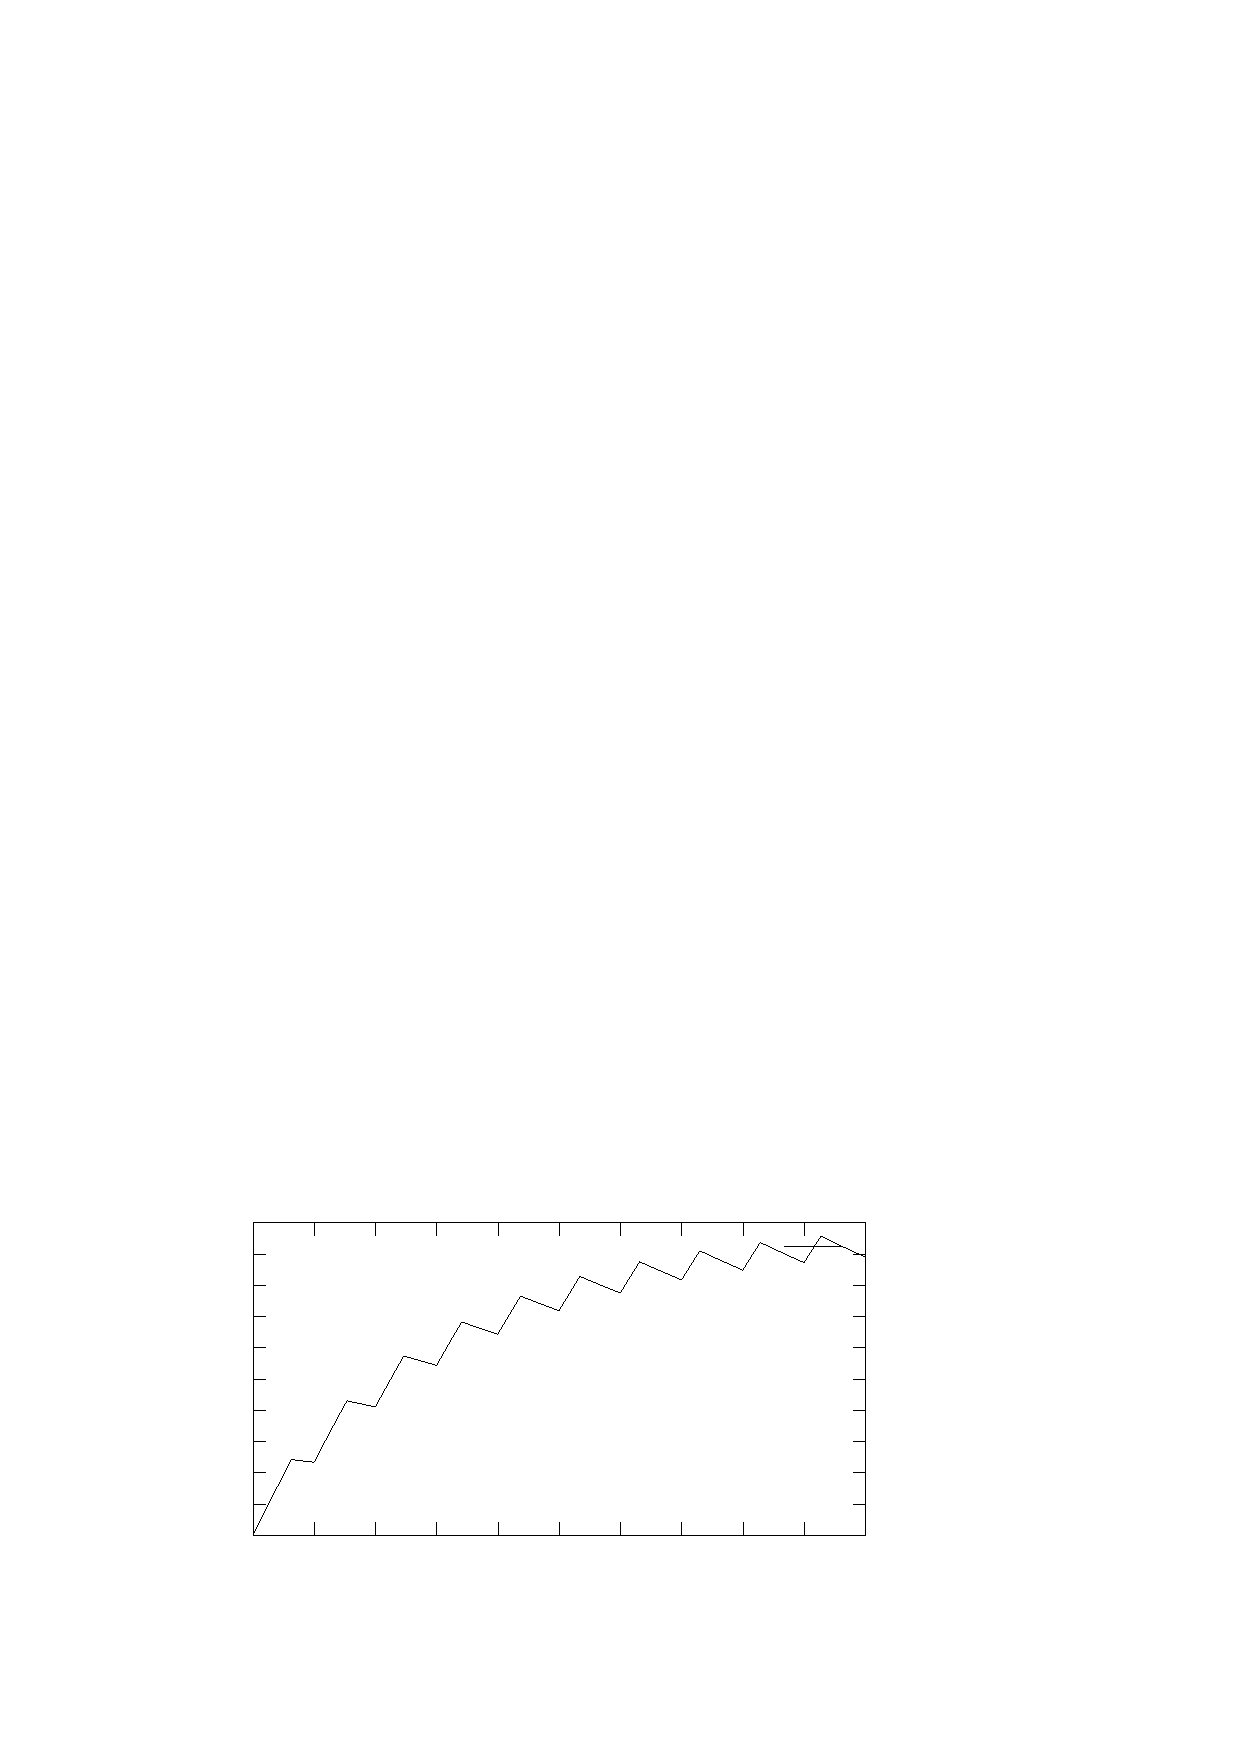
\includegraphics{CS}%
\end{picture}%
\begingroup
\setlength{\unitlength}{0.0200bp}%
\begin{picture}(18000,10800)(0,0)%
\put(2200,1650){\makebox(0,0)[r]{\strut{} 0}}%
\put(2200,2400){\makebox(0,0)[r]{\strut{} 0.5}}%
\put(2200,3150){\makebox(0,0)[r]{\strut{} 1}}%
\put(2200,3900){\makebox(0,0)[r]{\strut{} 1.5}}%
\put(2200,4650){\makebox(0,0)[r]{\strut{} 2}}%
\put(2200,5400){\makebox(0,0)[r]{\strut{} 2.5}}%
\put(2200,6150){\makebox(0,0)[r]{\strut{} 3}}%
\put(2200,6900){\makebox(0,0)[r]{\strut{} 3.5}}%
\put(2200,7650){\makebox(0,0)[r]{\strut{} 4}}%
\put(2200,8400){\makebox(0,0)[r]{\strut{} 4.5}}%
\put(2200,9150){\makebox(0,0)[r]{\strut{} 5}}%
\put(2475,1100){\makebox(0,0){\strut{} 0}}%
\put(3945,1100){\makebox(0,0){\strut{} 200}}%
\put(5415,1100){\makebox(0,0){\strut{} 400}}%
\put(6885,1100){\makebox(0,0){\strut{} 600}}%
\put(8355,1100){\makebox(0,0){\strut{} 800}}%
\put(9825,1100){\makebox(0,0){\strut{} 1000}}%
\put(11295,1100){\makebox(0,0){\strut{} 1200}}%
\put(12765,1100){\makebox(0,0){\strut{} 1400}}%
\put(14235,1100){\makebox(0,0){\strut{} 1600}}%
\put(15705,1100){\makebox(0,0){\strut{} 1800}}%
\put(17175,1100){\makebox(0,0){\strut{} 2000}}%
\put(550,5400){\rotatebox{0}{\makebox(0,0){\strut{}$I_L$}}}%
\put(9825,275){\makebox(0,0){\strut{}time ($10^{-7}s$)}}%
\put(9825,9975){\makebox(0,0){\strut{}switch circuit}}%
\end{picture}%
\endgroup
\endinput
  
 \end{figure}

 }
